\chapter{Preprocessamento}\label{pre}

\section{Coleta e Preprocessamento dos dados da PRF}\label{intro:metodologia}


As informações para suprir nosso modelo preditivo estão disponíveis na Internet, em sua maioria são Dados Governamentais Abertos, tais como os dados
da PRF, INPE e IBGE. Isto são iniciativas governamentais para fomentar a participação popular, dentro outros motivos, essas informações são também 
conhecidas como \textit{open data} \cite{DadosGoverno}, contudo os dados referentes à PRF e ao BPRv, para esta pesquisa, foram cedidos pelos respectivos 
órgãos governamentais (ver anexos) já em formato CSV para serem utilizados exclusivamente nesta pesquisa. Isso possibilitou ganho qualitativo nos dados evitando 
passar pelos transtornos como descreve Costa (2015) quando coletou os dados diretamente da Internet.\cite{Costa2015} 
As bases de dados do INPE e do base de dados do IBGE apresentaram boa qualidade o que justificou serem serem coletados diretamente da Internet.


\begin{table}[htbp!]
 \centering
  \caption{Variáveis originais da base de acidentes} 
  \begin{tabular}{r|l} \hline
   Ano & Ano da ocorrência do acidente\\
   Mês & Mês de ocorrência do acidente\\
   Num & Número do mês do acidente ex: 1 = Janeiro \\
   KM & Numeração do quilômetro \\
   BR & Numeração da Br\\
   Latitude & Latitude da ocorrência \\
   Longitude & Longitude da ocorrência \\
   Condição Pista & Condição da pista: seca, molhado, ... \\
   Restrição de Visibilidade & Restrição de visibilidade: inexistente, neblina, .., outros \\
   Tipo Acidente & Tipo de Acidente: atropelamento, colisão lateral,..\\
   Cauda Acidente & A possível causa do acidente: Falta de atenção, ... \\
   Sentido Via & Sentido da via: crescente, decrescente \\
   Traçado Via & Tipo de traçado da via: reta, curva, cruzamento, ... \\
   Município  & Localidade onde ocorreu \\
   Tipo veículo & Tipo de veículo envolvido no acidente \\
   Data Inversa & Data do acidente no formato dd/mm/aa \\
   Horário & Hora que ocorreu o acidente no formato hh/mm/ss \\
   Qtd Feridos Graves & Quantidade de feridos graves envolvidos \\
   Qtd Feridos Leves & Quantidade de feridos leves envolvidos\\
   Qtd Ilesos & Quantidade de ilesos envolvidos\\
   Qtd Mortos & Quantidade de mortos envolvidos \\
   Qtd Pessoas & Quantidade de pessoas envolvidos \\
   Qtd Veículos & Quantidade de veículos envolvidos\\
   Qtd Acidentes Graves & Quantidade de acidentes graves \\
   Qtd Ocorrências & Quantidade de ocorrências \\
  \end{tabular}
\end{table}

\pagebreak

Na tabela seguinte; as variáveis originais da base de dados da PRF com interdições das vias 
(somente interdições que paralisaram as BRs, não contém acidentes, exemplo: passeatas, protestos) 

\begin{table}[htbp]
 \centering
  \caption{Variáveis originais da base de interdições}
  
  \begin{tabular}{r|l} \hline
   Comunicação & Código do agente que comunicou o incidente \\
   Data Hora & Data hora no formato dd/mm/aa mm:ss \\
   BR & Numeração da Br do incidente\\
   KM & Numeração do quilômetro do incidente\\
   Trecho  & Local onde ocorreu o incidente \\
  \end{tabular}
\end{table}


\begin{figure}[ht]
  \centering
    \caption{Etapas 1 -- Coleta e união das bases históricas de acidentes e interdições}
    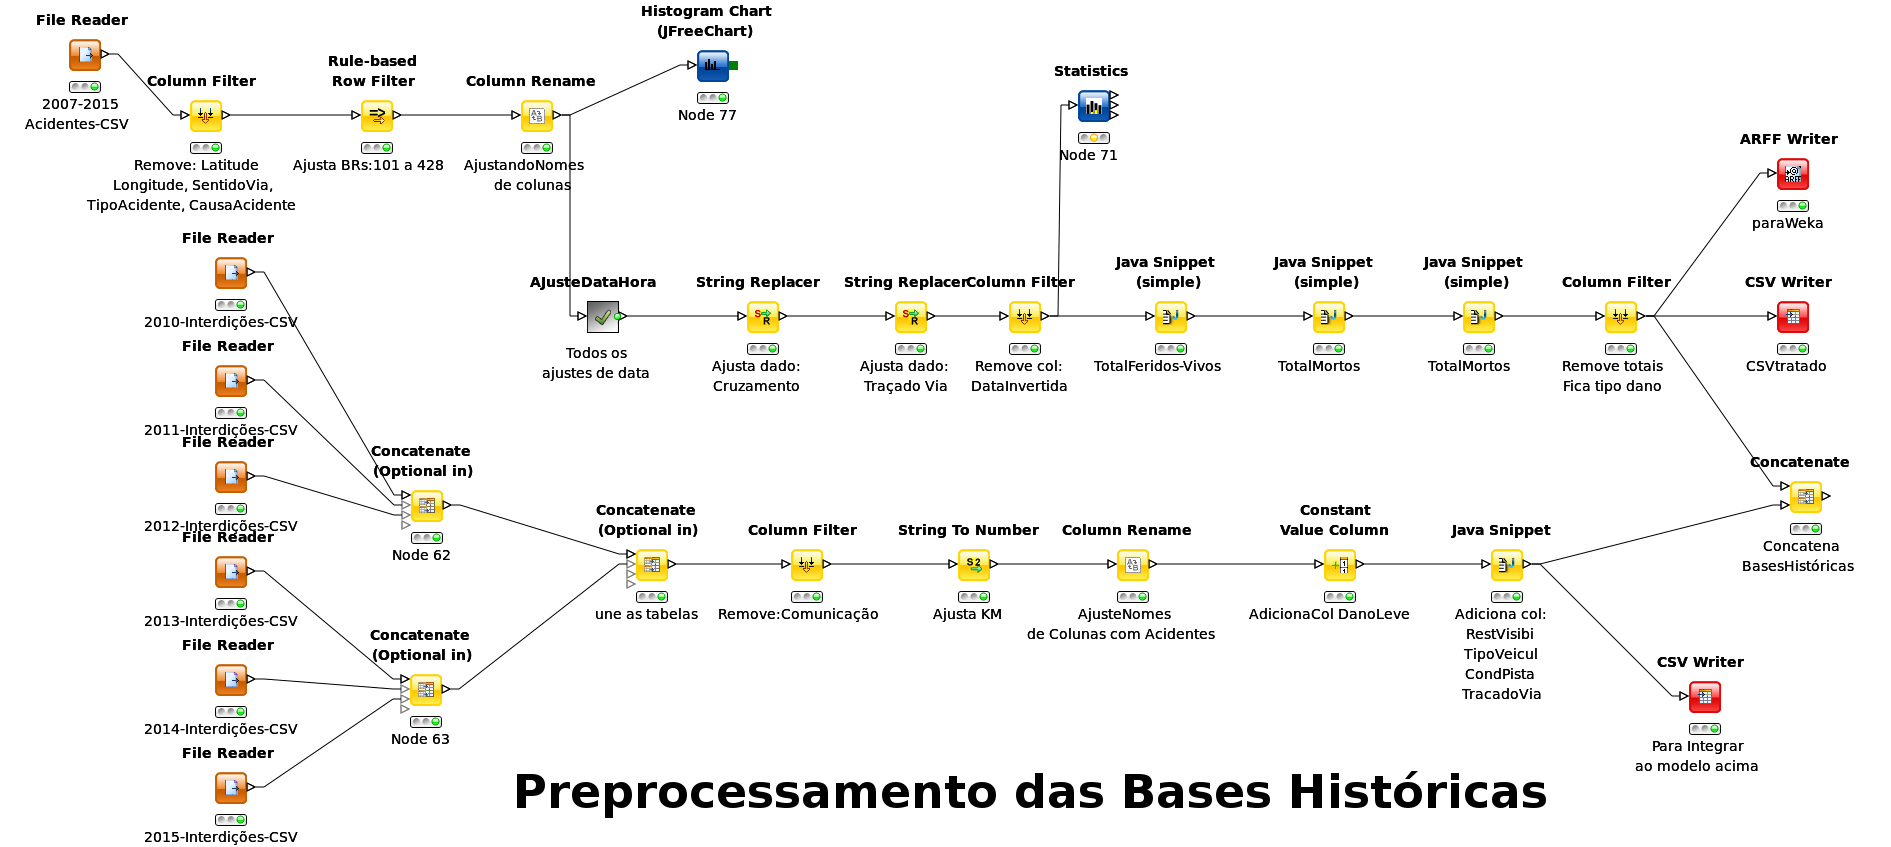
\includegraphics[width=165mm, height=100mm]{Figuras/Cronograma/BasesHistoricas.png}
\end{figure}